\subsection{\texorpdfstring{I$^2$C Features \& Overview}{I2C Features \& Overview}}
\label{chap:Back_I2C_Features_Overview}

Like other serial communication protocols, the I$^2$C bus has a serial data line 
(SDA) and a serial clock line (SCL). However, unlike other serial protocols, the I$^2$C 
protocol was created to allow communication between multiple devices over these 
two shared lines. The SCL line, mostly managed by the master device, serves to 
clock data in or out of the slave device. The other, the SDA line, sends or 
receives data to and from the slave devices. Figure~\ref{fig:i2c_imp} shows a standard I$^2$C 
physical layer implementation.


\begin{figure}[H]
    \centering
    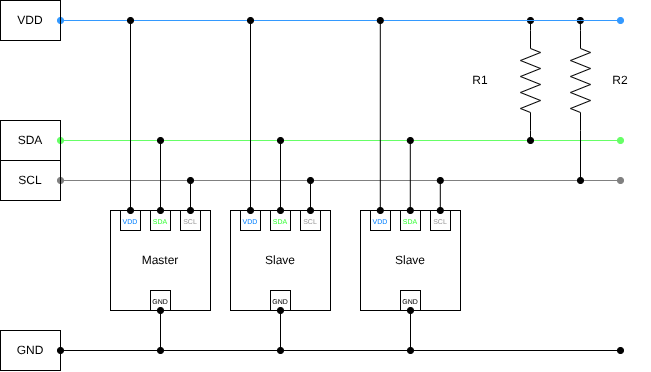
\includegraphics[width=1\textwidth]{Resources/Imagenes/typical_I2C.png}
    \caption{Typical I$^2$C implementation.}
    \label{fig:i2c_imp}
\end{figure}


The I$^2$C protocol is designed so that the SDA and SCL lines have an open-drain 
connection with all devices on the bus. This requires a pull-up resistor connected to 
a common voltage source, as shown in Figure~\ref{fig:i2c_imp}. The pull-up resistors define 
the high logic level and ensure that contention does not occur on the bus, where 
one device attempts to activate the line while another deactivates it. This prevents 
potential damage to the controllers.


\begin{figure}[H]
    \centering
    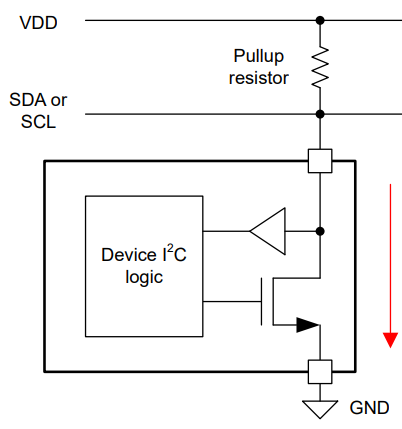
\includegraphics[width=0.5\textwidth]{Resources/Imagenes/open_drain.png}
    \caption{Open Drain.}
    \label{fig:i2c_open_drain}
\end{figure}


The I$^2$C protocol is designed as a half-duplex communication scheme, in which 
only a single master or slave device transmits data on the bus at any given time. 
Each device connected to the bus is identified by a unique address and can 
operate as either a transmitter or a receiver. During any given transaction, a simple 
master-slave relationship is established: masters can act as master-transmitters or 
master-receivers, where the master is the device that initiates the data transfer and generates 
the clock signals required for communication.


\begin{figure}[H]
    \centering
    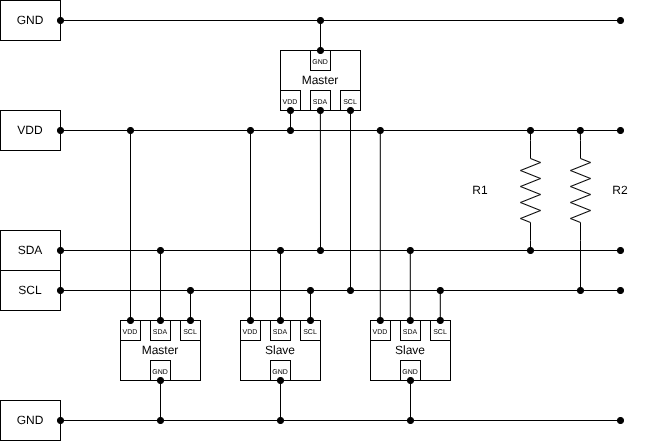
\includegraphics[width=0.7\textwidth]{Resources/Imagenes/i2c_multi_master.png}
    \caption{Multi-master example}
    \label{fig:i2c_multi_master}
\end{figure}


There can be more than one master connected to the same bus, both capable 
of controlling it. Since masters are usually microcontrollers, an example of data 
transfer between two microcontrollers connected to the I$^2$C bus is shown in Figure~\ref{fig:i2c_multi_master}. 
This example highlights the master-slave and transceiver roles that can 
arise on the I$^2$C bus. These roles are not permanent; they depend solely on which 
device initiates communication and the current direction of the data transfer.

A data transfer between two microcontrollers, A and B, proceeds as follows \cite{I2CSpec2000}:

\begin{enumerate}
    \item When microcontroller A wants to send information to microcontroller B:
    \begin{itemize}
        \item Microcontroller A (master) addresses microcontroller B (slave).
        \item Microcontroller A (master-transmitter) sends data to microcontroller B (slave-receiver).
        \item Microcontroller A terminates the transfer.
    \end{itemize}

    \item When microcontroller A wants to receive information from microcontroller B:
    \begin{itemize}
            \item Microcontroller A (master) addresses microcontroller B (slave).
            \item Microcontroller A (master-receiver) receives data from microcontroller B (slave-transmitter).
            \item Microcontroller A again terminates the transfer.
    \end{itemize}
\end{enumerate}

No matter the situation, even when he is the one receiving the information, the 
master (the microcontroller A in the example) generates the clock signal and ends 
the transfer, always.

When multiple microcontrollers are connected to the I$^2$C bus, more than one 
master may attempt to initiate a transfer at the same time. So, in order to prevent 
conflicts, an arbitration procedure is used, relying on the wired-AND\footnotemark[2] connection of 
all I$^2$C interfaces to the bus. If two or more masters attempt to place data on the 
bus simultaneously, the first master that attempts to transmit a logical "1" while 
another master drives a logical "0" will lose arbitration and must cease transmitting. 
During arbitration, the clock signals on SCL become a synchronized combination of 
the clocks generated by all contending masters through the wired-AND connection 
to the clock line.

\footnotetext[1]
{
    Half-duplex communication is a transmission mode where data can be sent and received in both 
    directions, but not simultaneously; only one party can transmit at a time, requiring the other to wait until 
    the transmission is complete before responding.
}

\footnotetext[2]
{
    It is type of logic gate that implements the Boolean AND operation using passive components such as 
    diodes and resistors, typically leveraging open collector or similar outputs
}